% =============================================================================
\bloco{3}{Created: the exam's economy, extended}{Kurlat \S\S6.2, 7.1, 9.1, 4.3; Romer \S2.9--2.11 \,\textbullet\, 28 points}

\questao{(15 points) \emph{The exam's household with leisure, inside an economy.} Periods $t=1,2,\dots$ Each period a generation of
size one is born and lives two periods, with one unit of time when young and none when old. Generation $t$ maximises
$\ln c_{1t}+\psi\ln(1-L_t)+\beta\ln c_{2t+1}$, $\psi>0$, $0<\beta<1$. Technology $Y_t=AK_t^\alpha L_t^{1-\alpha}$, $\delta=1$, competitive markets; saving is lent
to firms as next period's capital and earns $1+r_{t+1}=r^K_{t+1}$. \emph{Generation 1 is the exam's household:} it is born with assets
$a_0\ge0$ and owns the firm, which owns $K_1>0$, so in period 1 it receives the profit $\Pi_1=Y_1-w_1L_1$ besides its wage. From
period 2 on, the old rent their capital to firms, which earn zero profit; each young generation earns only its wage.}

\textbf{a)} (2 points) Write generation 1's two period budgets and its present-value budget constraint. List every choice variable
and every income source, and read the constraint in words.

\textbf{b)} (4 points) Derive all first-order conditions and closed forms for $c_1,c_2,L_1,a_1$ given $(w_1,\Pi_1,r_2,a_0)$. When is $L_1$
interior? Show that $a_1$ is the share $\frac{\beta}{1+\beta}$ of the resources $a_0+w_1L_1+\Pi_1$. What happens as $\psi\to0$?

\textbf{c)} (3 points) Let $a_0=0$. Using the firm's FOC, find equilibrium $L_1^\ast$ (show it depends on neither $K_1$ nor $A$) and the
map $K_2=\phi_1(K_1)$.

\textbf{d)} (3 points) For $t\ge2$ find the young's labour $\bar L$, the law of motion $K_{t+1}=\phi(K_t)$, the steady state and its stability.
Draw $\phi$ against the $45^\circ$ line for $\alpha=1/3$, $\beta=0.8$, $\psi=0.5$, $A=5$, $K_1=1$, marking $K^\ast$ and the path from $K_2$.

\textbf{e)} (3 points) Compare with Solow ($\delta$, $n$, $s$) and with $s_{GR}$. When does this economy over-accumulate? Evaluate for
$(\alpha,\beta)=(1/3,0.8)$ and $(0.2,0.9)$, with the interest rate in each. Why does generation 1 work less than later ones, and what goes
wrong if $\Pi_1$ is left out of its budget?
\resolespaco
\begin{sol}
\begin{notacao}
\item $c_{1t}$, $c_{2t+1}>0$: consumption of generation $t$ young and old (for generation 1: $c_1$, $c_2$). $L_t\in[0,1]$: hours of the
young; $1-L_t$: leisure. $\psi>0$: weight of leisure. $\beta\in(0,1)$: discount factor.
\item $Y_t=AK_t^\alpha L_t^{1-\alpha}$: output, $A>0$, $\alpha\in(0,1)$; $K_t$: capital, $\delta=1$.
\item $w_t$: wage. $r_{t+1}$: interest rate, $1+r_{t+1}=r^K_{t+1}$ (rental rate). $a_0\ge0$: generation 1's initial assets.
$a_1$ ($a_t$): saving of generation 1 ($t$). $\Pi_1=Y_1-w_1L_1$: period-1 profit.
\item $X$: full wealth; $R$: resources; $\lambda>0$: multiplier on the budget (defined where first used).
\item $L_1^\ast$: generation 1's equilibrium hours; $\bar L$: later generations' hours. $\phi_1$, $\phi$: laws of motion of capital;
$K^\ast$: steady state. $s_{eq}$: the equilibrium saving rate $K_{t+1}/Y_t$. $s_{GR}$: golden-rule rate.
\end{notacao}
\passo{(a)}{The two period budgets of generation 1:}
\begin{align}
c_1+a_1 &= a_0+w_1L_1+\Pi_1, \label{q9:b1}\\
c_2 &= (1+r_2)a_1. \label{q9:b2}
\end{align}
Solve \eqref{q9:b2} for $a_1=\frac{c_2}{1+r_2}$ and substitute into \eqref{q9:b1}:
\begin{equation}
c_1+\frac{c_2}{1+r_2}=a_0+w_1L_1+\Pi_1. \label{q9:pv}
\end{equation}
Add $w_1(1-L_1)$ to both sides of \eqref{q9:pv}:
\begin{equation}
c_1+\frac{c_2}{1+r_2}+w_1(1-L_1)=a_0+w_1+\Pi_1\equiv X. \label{q9:full}
\end{equation}
Choices: $c_1,c_2,a_1,L_1$ with $0\le L_1\le1$. Income: initial wealth, labour, \emph{and profits}. Reading: the present value of
consumption plus the value of leisure equals full wealth (time valued at $w_1$).
\passo{(b) FOCs}{The Lagrangian, with the budget \eqref{q9:pv}:}
\begin{equation}
\mathcal L=\ln c_1+\psi\ln(1-L_1)+\beta\ln c_2+\lambda\Big[a_0+w_1L_1+\Pi_1-c_1-\frac{c_2}{1+r_2}\Big]. \label{q9:lag}
\end{equation}
Differentiate \eqref{q9:lag} with respect to $c_1$, $c_2$ and $L_1$:
\begin{align}
\frac1{c_1} &= \lambda, \label{q9:f1}\\
\frac\beta{c_2} &= \frac\lambda{1+r_2}, \label{q9:f2}\\
\frac\psi{1-L_1} &= \lambda w_1. \label{q9:f3}
\end{align}
Substitute \eqref{q9:f1} into \eqref{q9:f2} (Euler) and into \eqref{q9:f3} (labour supply):
\begin{align}
\frac\beta{c_2} &= \frac{(1/c_1)}{1+r_2}\nonumber\\
c_2 &= \beta(1+r_2)c_1, \label{q9:euler}\\
\frac\psi{1-L_1} &= \Big(\frac1{c_1}\Big)w_1\nonumber\\
w_1(1-L_1) &= \psi c_1. \label{q9:ls}
\end{align}
\passo{(b) closed forms}{Substitute \eqref{q9:euler} and \eqref{q9:ls} into the full budget \eqref{q9:full}:}
\begin{align*}
c_1+\frac{\big(\beta(1+r_2)c_1\big)}{1+r_2}+(\psi c_1) &= X\\
c_1+\beta c_1+\psi c_1 &= X,
\end{align*}
so
\begin{equation}
c_1=\frac{X}{1+\beta+\psi}. \label{q9:c1}
\end{equation}
Substitute \eqref{q9:c1} into \eqref{q9:euler}, into \eqref{q9:ls} solved for $L_1$, and into $a_1=\frac{c_2}{1+r_2}$:
\begin{align}
c_2 &= \beta(1+r_2)\Big(\frac{X}{1+\beta+\psi}\Big)\nonumber\\
&= \frac{\beta(1+r_2)X}{1+\beta+\psi}, \nonumber\\
L_1 &= 1-\frac{\psi}{w_1}\Big(\frac{X}{1+\beta+\psi}\Big)\nonumber\\
&= 1-\frac{\psi X}{(1+\beta+\psi)w_1}, \label{q9:L1}\\
a_1 &= \frac1{1+r_2}\Big(\frac{\beta(1+r_2)X}{1+\beta+\psi}\Big)\nonumber\\
&= \frac{\beta X}{1+\beta+\psi}. \label{q9:a1}
\end{align}
Interior iff $L_1>0$. By \eqref{q9:L1} and the definition of $X$ in \eqref{q9:full}:
\begin{align}
L_1>0 &\iff 1-\frac{\psi(a_0+w_1+\Pi_1)}{(1+\beta+\psi)w_1}>0\nonumber\\
&\iff \psi(a_0+w_1+\Pi_1)<(1+\beta+\psi)w_1\nonumber\\
&\iff \psi(a_0+\Pi_1)<(1+\beta)w_1. \label{q9:int}
\end{align}
\passo{(b) saving share}{Resources are full wealth minus the value of leisure, \eqref{q9:full}; then use \eqref{q9:ls} and \eqref{q9:c1}:}
\begin{align}
R\equiv a_0+w_1L_1+\Pi_1 &= X-w_1(1-L_1)\nonumber\\
&= X-(\psi c_1)\nonumber\\
&= X-\psi\Big(\frac{X}{1+\beta+\psi}\Big)\nonumber\\
&= X-\frac{\psi X}{1+\beta+\psi}\nonumber\\
&= \frac{(1+\beta)X}{1+\beta+\psi}. \label{q9:R}
\end{align}
Divide \eqref{q9:a1} by \eqref{q9:R}:
\begin{align*}
\frac{a_1}{R} &= \frac{\big(\beta X/(1+\beta+\psi)\big)}{\big((1+\beta)X/(1+\beta+\psi)\big)}\\
&= \frac{\beta}{1+\beta},
\end{align*}
the exam's rate, for any $\psi$ and any $r_2$. As $\psi\to0$, \eqref{q9:L1} and \eqref{q9:c1} give
\begin{align*}
L_1 &\to 1-\frac{(0)X}{(1+\beta+(0))w_1}=1\quad\text{(the exam's corner)},\\
c_1 &\to \frac{(a_0+w_1+\Pi_1)}{1+\beta+(0)}=\frac{a_0+w_1+\Pi_1}{1+\beta}.
\end{align*}
\passo{(c) labour}{The firm's FOC for labour, and profit as output minus wages:}
\begin{align}
w_1 &= (1-\alpha)AK_1^\alpha L_1^{-\alpha}=\frac{(1-\alpha)Y_1}{L_1}, \label{q9:w}\\
\Pi_1 &= Y_1-w_1L_1=\alpha Y_1. \label{q9:Pi}
\end{align}
With $a_0=0$, \eqref{q9:full} and \eqref{q9:Pi} give $X=(0)+w_1+(\alpha Y_1)=w_1+\alpha Y_1$. Multiply \eqref{q9:L1} out as
$w_1(1-L_1)=\frac{\psi X}{1+\beta+\psi}$ and substitute \eqref{q9:w} and $X$:
\begin{align*}
\Big(\frac{(1-\alpha)Y_1}{L_1}\Big)(1-L_1) &= \frac{\psi}{1+\beta+\psi}\Big[\Big(\frac{(1-\alpha)Y_1}{L_1}\Big)+\alpha Y_1\Big]\\
\frac{(1-\alpha)Y_1(1-L_1)}{L_1} &= \frac{\psi}{1+\beta+\psi}\Big[\frac{(1-\alpha)Y_1}{L_1}+\alpha Y_1\Big].
\end{align*}
Multiply by $\frac{L_1(1+\beta+\psi)}{Y_1}$:
\[
(1-\alpha)(1+\beta+\psi)(1-L_1)=\psi(1-\alpha)+\psi\alpha L_1 .
\]
Collect the $L_1$ terms on the right; $\psi(1-\alpha)$ cancels on the left:
\[
(1-\alpha)(1+\beta)=L_1\big[(1-\alpha)(1+\beta)+\psi\big].
\]
Hence
\begin{equation}
L_1^\ast=\frac{(1-\alpha)(1+\beta)}{(1-\alpha)(1+\beta)+\psi}. \label{q9:Lstar}
\end{equation}
$Y_1$ cancelled, so $K_1$ and $A$ drop out. Interiority: \eqref{q9:int} with $a_0=0$, then \eqref{q9:w}--\eqref{q9:Pi}, then
\eqref{q9:Lstar}:
\begin{align*}
\psi\Pi_1<(1+\beta)w_1 &\iff \psi(\alpha Y_1)<(1+\beta)\Big(\frac{(1-\alpha)Y_1}{L_1^\ast}\Big)\\
&\iff \psi\alpha L_1^\ast<(1-\alpha)(1+\beta)\\
&\iff \psi\alpha\Big(\frac{(1-\alpha)(1+\beta)}{(1-\alpha)(1+\beta)+\psi}\Big)<(1-\alpha)(1+\beta)\\
&\iff \psi\alpha<(1-\alpha)(1+\beta)+\psi,
\end{align*}
always true.
\passo{(c) map}{With $a_0=0$, \eqref{q9:w}--\eqref{q9:Pi} give $R=w_1L_1+\Pi_1=\big(\frac{(1-\alpha)Y_1}{L_1}\big)L_1+(\alpha Y_1)=Y_1$. Capital is
the only asset, so market clearing is}
\begin{equation}
K_2=a_1. \label{q9:mc}
\end{equation}
Substitute $a_1=\frac{\beta}{1+\beta}R=\frac{\beta}{1+\beta}Y_1$ and $L_1=L_1^\ast$ into \eqref{q9:mc}:
\begin{align}
K_2 &= \Big(\frac{\beta}{1+\beta}Y_1\Big)\nonumber\\
&= \frac{\beta}{1+\beta}\big(AK_1^\alpha(L_1^\ast)^{1-\alpha}\big)\nonumber\\
&= \frac{\beta}{1+\beta}AK_1^\alpha(L_1^\ast)^{1-\alpha}\equiv\phi_1(K_1). \label{q9:phi1}
\end{align}
\passo{(d) later generations}{$a_0=\Pi=0$, so \eqref{q9:full} gives $X=(0)+w_t+(0)=w_t$, and \eqref{q9:L1} becomes}
\begin{align}
\bar L &= 1-\frac{\psi(w_t)}{(1+\beta+\psi)w_t}\nonumber\\
&= 1-\frac{\psi}{1+\beta+\psi}=\frac{1+\beta}{1+\beta+\psi}. \label{q9:Lbar}
\end{align}
Saving is the share $\frac{\beta}{1+\beta}$ of resources $w_t\bar L$, and $w_t\bar L=(1-\alpha)Y_t$ by \eqref{q9:w}:
\begin{equation}
a_t=\frac{\beta}{1+\beta}w_t\bar L=\frac{\beta}{1+\beta}\big((1-\alpha)Y_t\big). \label{q9:at}
\end{equation}
Market clearing $K_{t+1}=a_t$, with $Y_t=AK_t^\alpha\bar L^{1-\alpha}$ in \eqref{q9:at}:
\begin{align}
K_{t+1} &= \frac{\beta}{1+\beta}(1-\alpha)\big(AK_t^\alpha\bar L^{1-\alpha}\big)\nonumber\\
\phi(K) &= \frac{\beta(1-\alpha)}{1+\beta}A\bar L^{1-\alpha}K^\alpha. \label{q9:phi}
\end{align}
$\phi(0)=0$, $\phi'>0$, $\phi''<0$, $\phi'(0^+)=\infty$, $\phi'(\infty)=0$: one positive fixed point. Set $\phi(K)=K$ in \eqref{q9:phi}, divide
by $K^\alpha$ and raise to the power $\frac1{1-\alpha}$:
\begin{align}
\frac{\beta(1-\alpha)}{1+\beta}A\bar L^{1-\alpha}K^\alpha &= (K)\nonumber\\
K^{1-\alpha} &= \frac{\beta(1-\alpha)A\bar L^{1-\alpha}}{1+\beta}\nonumber\\
K^\ast &= \Big[\frac{\beta(1-\alpha)A\bar L^{1-\alpha}}{1+\beta}\Big]^{\frac1{1-\alpha}}. \label{q9:Kstar}
\end{align}
Differentiating \eqref{q9:phi}, $\phi'(K^\ast)=\alpha\frac{\phi(K^\ast)}{K^\ast}=\alpha\frac{(K^\ast)}{K^\ast}=\alpha<1$: monotone, stable.
\passo{(d) numbers}{With $\alpha=1/3$, $\beta=0.8$, $\psi=0.5$, $A=5$, $K_1=1$:}
\begin{align*}
\bar L &= \tfrac{1+0.8}{1+0.8+0.5}=1.8/2.3=0.7826 &&\text{by \eqref{q9:Lbar}},\\
L_1^\ast &= \tfrac{(2/3)(1.8)}{(2/3)(1.8)+0.5}=1.2/1.7=0.7059 &&\text{by \eqref{q9:Lstar}},\\
\phi(K) &= \tfrac{0.8\cdot2/3}{1.8}\cdot5\cdot0.7826^{2/3}K^{1/3}=1.2581K^{1/3} &&\text{by \eqref{q9:phi}},\\
K^\ast &= 1.2581^{1.5}=1.4112 &&\text{by \eqref{q9:Kstar}},\\
Y_1 &= 5\cdot(1)^{1/3}\cdot0.7059^{2/3}=3.9639,\\
K_2 &= \tfrac{0.8}{1.8}\times3.9639=1.7617 &&\text{by \eqref{q9:phi1}}.
\end{align*}
Then \eqref{q9:phi} gives $K_3=1.2581\,(1.7617)^{1/3}=1.5195$ and, iterating the same way, $K_4=1.4464$, $K_5=1.4228\to K^\ast$.
\begin{center}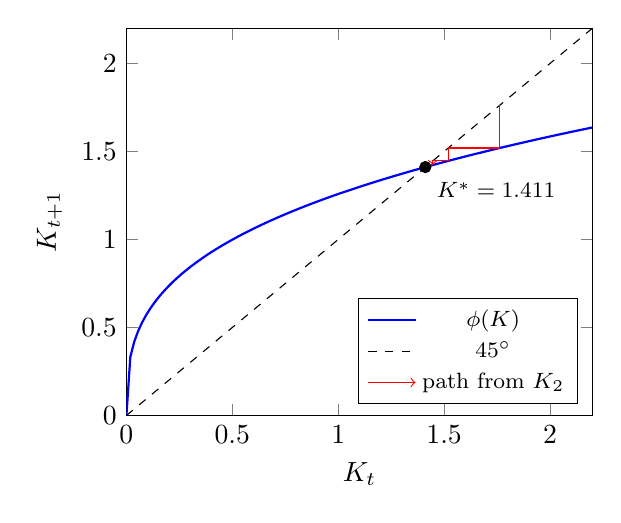
\begin{tikzpicture}\begin{axis}[width=7.5cm,height=6.5cm,xmin=0,xmax=2.2,ymin=0,ymax=2.2,xlabel={$K_t$},ylabel={$K_{t+1}$},
legend pos=south east,legend style={font=\footnotesize},samples=120,domain=0:2.2]
\addplot[blue,thick] {1.2581*x^(1/3)};
\addplot[black,dashed] {x};
\addplot[red,thin,->] coordinates {(1.7617,1.7617) (1.7617,1.5195) (1.5195,1.5195) (1.5195,1.4464) (1.4464,1.4464) (1.4464,1.4228)};
\addplot[only marks,mark=*] coordinates {(1.4112,1.4112)};
\legend{$\phi(K)$, $45^\circ$, path from $K_2$}
\node[anchor=north west,font=\footnotesize] at (axis cs:1.42,1.38) {$K^\ast=1.411$};
\end{axis}\end{tikzpicture}\end{center}
\passo{(e) Solow}{With $\delta=1$, $n=0$ Solow's law of motion is}
\begin{equation}
K_{t+1}=sY_t. \label{q9:solow}
\end{equation}
Here, by market clearing and \eqref{q9:at},
\begin{equation}
\frac{K_{t+1}}{Y_t}=\frac{\beta(1-\alpha)}{1+\beta}\equiv s_{eq}: \label{q9:seq}
\end{equation}
the same law of motion as \eqref{q9:solow}, but $s$ is chosen (patience, and the wage share because only wages are saved), and it
need not be $s_{GR}=\alpha$. Golden rule: MPK $=n+\delta=1$. At $K^\ast$, $K=s_{eq}Y$ by \eqref{q9:seq}, so
\begin{align}
1+r=\text{MPK} &= \alpha\frac YK\nonumber\\
&= \alpha\frac{Y}{(s_{eq}Y)}\nonumber\\
&= \frac{\alpha}{s_{eq}}. \label{q9:r}
\end{align}
By \eqref{q9:r}, and multiplying out \eqref{q9:seq} as in Question~7(c):
\begin{align*}
r<0=n &\iff s_{eq}>\alpha\\
&\iff \frac{\beta(1-\alpha)}{1+\beta}>\alpha\\
&\iff \beta(1-2\alpha)>\alpha .
\end{align*}
\passo{(e) numbers}{Using \eqref{q9:seq} and \eqref{q9:r}:}
\begin{align*}
(1/3,0.8) &: \ s_{eq}=\tfrac{0.8\times2/3}{1.8}=0.2963<0.3333,\quad 1+r=\tfrac{1/3}{0.2963}=1.125,\quad r=0.125>0,\\
(0.2,0.9) &: \ s_{eq}=\tfrac{0.9\times0.8}{1.9}=0.3789>0.2,\quad 1+r=\tfrac{0.2}{0.3789}=0.5278,\quad r=-0.472<0.
\end{align*}
The first is under-accumulation, efficient; the second is over-accumulation, dynamically inefficient.
\passo{(e) profits}{Compare \eqref{q9:Lstar} with \eqref{q9:Lbar}; cross-multiply and cancel $(1-\alpha)(1+\beta)$:}
\begin{align*}
L_1^\ast<\bar L &\iff \frac{(1-\alpha)(1+\beta)}{(1-\alpha)(1+\beta)+\psi}<\frac{1+\beta}{1+\beta+\psi}\\
&\iff (1-\alpha)(1+\beta+\psi)<(1-\alpha)(1+\beta)+\psi\\
&\iff (1-\alpha)\psi<\psi,
\end{align*}
true. Profits are non-labour income; the wealth effect buys leisure. Dropping $\Pi_1$ gives $L_1=\bar L$ and
$K_2=\frac{\beta}{1+\beta}(1-\alpha)Y_1$: it understates resources by $\alpha Y_1$ and overstates labour.
\intuicao{The household rule is the same in every generation; what differs is who owns what. Market clearing turns that rule into
$\phi$, and the saving rate it implies answers to preferences and factor shares, not to the golden rule.}
\refbib{Kurlat (2020), \S6.2 (Euler), \S7.1 (labour supply), \S9.1 (two-period equilibrium), \S4.3 (golden rule); Romer (2012), \S\S2.9--2.11.
Same structure as Prova 01, Q2(c)--(f), with $\psi=0$; see \texttt{Prova/prova-01-error-analysis.md}.}
\rubrica{
\item (a): 2 pts; $\Pi_1$ missing: max.\ 1 pt. (b) all four FOCs (or three plus the corner argument): 2 pts; closed forms and $\beta/(1+\beta)$: 2 pts.
\item (c): 3 pts. (d): 3 pts, of which the diagram 1 pt (axes, $45^\circ$ line, curve, $K^\ast$ and direction marked separately: 0.25 each).
\item (e): 3 pts. Ceiling: no market clearing ($K_{t+1}=a_t$) anywhere: max.\ 6 pts for the whole question.
}
\end{sol}

% -----------------------------------------------------------------------------
\questao{(13 points) \emph{CRRA and population growth: when the saving rate depends on $r$.} Overlapping generations as in
Question~9 but without leisure: each young person supplies one unit of labour, earns only the wage, and the number of young grows,
$L_{t+1}=(1+n)L_t$. Utility $u(c_{1t})+\beta u(c_{2t+1})$ with $u(c)=\frac{c^{1-\sigma}}{1-\sigma}$; $y=Ak^\alpha$ per young worker; $\delta=1$.}

\textbf{a)} (3 points) Solve the young's problem. Show that saving is a share $s(r)$ of the wage, find $s(r)$, and sign $s'(r)$.
Explain the sign through income and substitution effects.

\textbf{b)} (3 points) Using the firm's FOCs and market clearing $K_{t+1}=L_ta_t$, write the law of motion for $k\equiv K/L$. Show that $k_{t+1}$
is unique given $k_t$ when $\sigma\le1$, and give it in closed form for $\sigma=1$.

\textbf{c)} (3 points) Show that the steady state satisfies $s(r)(1+r)=\frac{\alpha(1+n)}{1-\alpha}$ and that the aggregate saving rate is
$\frac{I}{Y}=\frac{\alpha(1+n)}{1+r}$. Conclude: $\frac IY>s_{GR}\iff r<n\iff k^\ast>k_{GR}$.

\textbf{d)} (2 points) Let $\alpha=0.2$, $\beta=0.5$, $n=0.3$, $A=5$. For $\sigma=1$ find $r^\ast$, $k^\ast$, $k_{GR}$ and steady-state consumption per
worker at both. For $\sigma\in\{1/2,2\}$ find $r^\ast$ numerically (Python) and say which economies are dynamically inefficient, and why
$\sigma$ matters.

\textbf{e)} (2 points) Draw the $\sigma=1$ map against the $45^\circ$ line, marking $k^\ast$ and $k_{GR}$. In what sense is this ``Solow with $\delta=1$''?
\resolespaco
\begin{sol}
\begin{notacao}
\item $c_1$, $c_2>0$: consumption young and old. $w$: wage. $a$: saving of a young person. $r>-1$: interest rate; $r^K$: rental rate.
\item $u(c)=\frac{c^{1-\sigma}}{1-\sigma}$, $\sigma>0$ ($1/\sigma$: intertemporal elasticity). $\beta\in(0,1)$: discount factor.
\item $D$: the consumption divisor, as in Question~3, \eqref{q3:D}. $s(r)$: share of the wage saved.
\item $L_t$: number of young, growing at rate $n>-1$. $k\equiv K/L$: capital per young worker; $y=Ak^\alpha$, $A>0$, $\alpha\in(0,1)$;
$\delta=1$.
\item $I/Y$: aggregate saving (investment) rate. $k^\ast$, $r^\ast$: steady state. $k_{GR}$, $s_{GR}$: golden rule. $H(r)$: the
steady-state residual of (d). $\phi(k)$: the law of motion; $s_S$: Solow's saving rate that reproduces it.
\end{notacao}
\passo{(a)}{The young person's two budgets:}
\begin{align}
c_1+a &= w, \label{q10:b1}\\
c_2 &= (1+r)a. \label{q10:b2}
\end{align}
The Euler equation is \eqref{q3:euler}, $c_2=[\beta(1+r)]^{1/\sigma}c_1$. Eliminating $a$ from \eqref{q10:b1}--\eqref{q10:b2} gives the PV
budget
\begin{equation}
c_1+\frac{c_2}{1+r}=w. \label{q10:pv}
\end{equation}
\eqref{q10:pv} is \eqref{q3:pv} with $W=w$, so, as in \eqref{q3:c1},
\begin{equation}
c_1=\frac wD,\qquad D=1+\beta^{1/\sigma}(1+r)^{\frac1\sigma-1}. \label{q10:c1}
\end{equation}
Substitute \eqref{q10:c1} into \eqref{q10:b1}:
\begin{align}
\Big(\frac wD\Big)+a &= w\nonumber\\
a &= w-\frac wD=s(r)w, \label{q10:a}
\end{align}
with
\begin{align}
s(r) &= \frac{D-1}{D}\nonumber\\
&= \frac{\big(1+\beta^{1/\sigma}(1+r)^{\frac1\sigma-1}\big)-1}{\big(1+\beta^{1/\sigma}(1+r)^{\frac1\sigma-1}\big)}\nonumber\\
&= \frac{\beta^{1/\sigma}(1+r)^{\frac1\sigma-1}}{1+\beta^{1/\sigma}(1+r)^{\frac1\sigma-1}}. \label{q10:s}
\end{align}
Write \eqref{q10:s} as $s=1-1/D$ and differentiate, with $D'(r)$ from \eqref{q3:Dr}:
\begin{equation}
s'(r)=\frac{D'(r)}{D^2},\qquad D'(r)=\beta^{1/\sigma}\Big(\frac1\sigma-1\Big)(1+r)^{\frac1\sigma-2}. \label{q10:ds}
\end{equation}
The sign of \eqref{q10:ds} is the sign of $1-\sigma$. The young are pure savers: a higher $r$ makes them richer ($c_1\uparrow$, saving
$\downarrow$) and makes waiting cheaper (saving $\uparrow$). $\sigma<1$: substitution wins; $\sigma>1$: income wins; $\sigma=1$:
\eqref{q10:s} gives
\begin{align*}
s &= \frac{\beta^{1/(1)}(1+r)^{\frac1{(1)}-1}}{1+\beta^{1/(1)}(1+r)^{\frac1{(1)}-1}}\\
&= \frac\beta{1+\beta},
\end{align*}
independent of $r$.
\passo{(b)}{The firm's FOCs, with $\delta=1$ so that $1+r=r^K$:}
\begin{align}
w_t &= (1-\alpha)Ak_t^\alpha, \label{q10:w}\\
1+r_{t+1} &= r^K_{t+1}=\alpha Ak_{t+1}^{\alpha-1}. \label{q10:r}
\end{align}
Market clearing:
\begin{equation}
K_{t+1}=L_ta_t. \label{q10:mc}
\end{equation}
Divide \eqref{q10:mc} by $L_{t+1}=(1+n)L_t$ and use \eqref{q10:a}:
\[
(1+n)k_{t+1}=a_t=s(r_{t+1})w_t .
\]
Substitute \eqref{q10:w} and \eqref{q10:r}:
\begin{equation}
(1+n)k_{t+1}=s\big(\alpha Ak_{t+1}^{\alpha-1}-1\big)(1-\alpha)Ak_t^\alpha. \label{q10:lom}
\end{equation}
The left side of \eqref{q10:lom} rises from 0 to $\infty$ in $k_{t+1}$; when $\sigma\le1$ the right side is positive and non-increasing in
$k_{t+1}$ (higher $k_{t+1}$, lower $r$, $s$ weakly lower by \eqref{q10:ds}): one crossing. $\sigma=1$: $s=\frac\beta{1+\beta}$ in
\eqref{q10:lom}, divided by $1+n$:
\begin{align}
(1+n)k_{t+1} &= \Big(\frac\beta{1+\beta}\Big)(1-\alpha)Ak_t^\alpha\nonumber\\
k_{t+1} &= \frac{\beta(1-\alpha)A}{(1+\beta)(1+n)}k_t^\alpha. \label{q10:lom1}
\end{align}
\passo{(c)}{Steady state: set $k_{t+1}=k_t=k$ in \eqref{q10:lom} and divide by $k^\alpha$:}
\begin{align}
(1+n)(k) &= s\big(\alpha A(k)^{\alpha-1}-1\big)(1-\alpha)A(k)^\alpha\nonumber\\
(1+n)k^{1-\alpha} &= s(r)(1-\alpha)A. \label{q10:ss1}
\end{align}
Solve \eqref{q10:r} for $k^{1-\alpha}$:
\begin{equation}
k^{1-\alpha}=\frac{\alpha A}{1+r}. \label{q10:k}
\end{equation}
Substitute \eqref{q10:k} into \eqref{q10:ss1}:
\begin{align}
(1+n)\Big(\frac{\alpha A}{1+r}\Big) &= s(r)(1-\alpha)A\nonumber\\
\frac{(1+n)\alpha A}{1+r} &= s(r)(1-\alpha)A\nonumber\\
s(r)(1+r) &= \frac{\alpha(1+n)}{1-\alpha}. \label{q10:ssr}
\end{align}
Gross investment is $K_{t+1}$ ($\delta=1$), which per young worker of period $t$ is $(1+n)k$. Divide by $y=Ak^\alpha$, then use
\eqref{q10:k}:
\begin{align}
\frac IY &= \frac{(1+n)k}{Ak^\alpha}\nonumber\\
&= \frac{(1+n)k^{1-\alpha}}{A}\nonumber\\
&= \frac{1+n}{A}\Big(\frac{\alpha A}{1+r}\Big)\nonumber\\
&= \frac{\alpha(1+n)}{1+r}. \label{q10:IY}
\end{align}
By \eqref{q10:ssr}, \eqref{q10:IY} also equals
\[
\frac IY=\frac{\big((1-\alpha)s(r)(1+r)\big)}{1+r}=(1-\alpha)s(r).
\]
Golden rule: MPK $=n+\delta=1+n$; by \eqref{q10:r} that is $1+r=1+n$,
where \eqref{q10:IY} gives $\frac IY=\frac{\alpha(1+n)}{(1+n)}=\alpha=s_{GR}$. As $\frac IY$ falls in $r$ and MPK falls in $k$:
$\frac IY>\alpha\iff r<n\iff k^\ast>k_{GR}$.
\passo{(d) $\sigma=1$}{With $s=\frac{\beta}{1+\beta}$, solve \eqref{q10:ssr} for $1+r$:}
\begin{align*}
\Big(\frac\beta{1+\beta}\Big)(1+r^\ast) &= \frac{\alpha(1+n)}{1-\alpha}\\
1+r^\ast &= \frac{\alpha(1+n)(1+\beta)}{(1-\alpha)\beta}=\frac{0.2\times1.3\times1.5}{0.8\times0.5}=0.975 .
\end{align*}
So $r^\ast=-0.025<n=0.3$: over-accumulation. By \eqref{q10:IY}:
\[
\frac IY=\frac{(0.2)(1.3)}{(0.975)}=\frac{0.26}{0.975}=0.2667>0.2 .
\]
The fixed point of \eqref{q10:lom1}, and \eqref{q10:k} at $r=n$:
\begin{align*}
k^\ast &= \Big(\frac{0.5\times0.8\times5}{1.5\times1.3}\Big)^{1.25}=1.0256^{1.25}=1.0322,\\
k_{GR} &= \Big(\frac{\alpha A}{1+n}\Big)^{1.25}=\Big(\frac{(0.2)(5)}{1+(0.3)}\Big)^{1.25}=(1/1.3)^{1.25}=0.7204.
\end{align*}
Steady-state consumption per worker is output minus the investment that keeps $k$ constant:
\begin{equation}
c=Ak^\alpha-(1+n)k. \label{q10:c}
\end{equation}
Evaluating \eqref{q10:c}:
\begin{align*}
c(k^\ast) &= 5(1.0322)^{0.2}-1.3(1.0322)=3.6899,\\
c(k_{GR}) &= 5(0.7204)^{0.2}-1.3(0.7204)=3.7461,
\end{align*}
so $c(k^\ast)<c(k_{GR})$.
\passo{(d) other $\sigma$}{Write \eqref{q10:ssr} as a root problem:}
\begin{equation}
H(r)=(1-\alpha)s(r)(1+r)-\alpha(1+n)=0. \label{q10:H}
\end{equation}
Solve \eqref{q10:H} by bisection on $(-0.99,49)$ (one sign change on a grid), and evaluate \eqref{q10:IY}:
\begin{align*}
\sigma=1/2 &: \ r^\ast=0.314>n,\quad \tfrac IY=0.198<0.2\ \text{(efficient)},\\
\sigma=2 &: \ r^\ast=-0.287<n,\quad \tfrac IY=0.365\ \text{(inefficient)}.
\end{align*}
With high $\sigma$ the young save \emph{more} when $r$ is low, which pushes $k$ up and $r$ further down; with low $\sigma$ low returns
discourage saving and hold $k$ back.
\passo{(e)}{With the numbers of (d), \eqref{q10:lom1} is $\phi(k)=1.0256k^{0.2}$. It crosses the $45^\circ$ line at $k^\ast=1.032$, to the
right of $k_{GR}=0.720$; from $k_0=0.3$: $0.806$, $0.982$, $1.022$, $1.030$.}
\begin{center}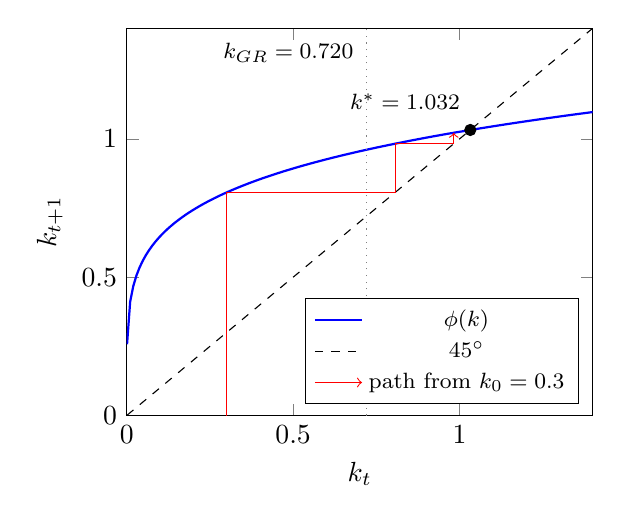
\begin{tikzpicture}\begin{axis}[width=7.5cm,height=6.5cm,xmin=0,xmax=1.4,ymin=0,ymax=1.4,xlabel={$k_t$},ylabel={$k_{t+1}$},
legend pos=south east,legend style={font=\footnotesize},samples=150,domain=0.001:1.4]
\addplot[blue,thick] {1.0256*x^(0.2)};
\addplot[black,dashed] {x};
\addplot[red,thin,->] coordinates {(0.3,0) (0.3,0.8062) (0.8062,0.8062) (0.8062,0.9824) (0.9824,0.9824) (0.9824,1.0220)};
\addplot[only marks,mark=*] coordinates {(1.0322,1.0322)};
\addplot[gray,dotted] coordinates {(0.7204,0) (0.7204,1.4)};
\legend{$\phi(k)$, $45^\circ$, path from $k_0=0.3$}
\node[anchor=north east,font=\footnotesize] at (axis cs:0.71,1.38) {$k_{GR}=0.720$};
\node[anchor=south east,font=\footnotesize] at (axis cs:1.03,1.07) {$k^\ast=1.032$};
\end{axis}\end{tikzpicture}\end{center}
Solow's discrete law with $\delta=1$ is
\begin{equation}
k_{t+1}=\frac{s_SAk_t^\alpha}{1+n}. \label{q10:solow}
\end{equation}
\eqref{q10:lom1} is \eqref{q10:solow} with $s_S=\frac{(1-\alpha)\beta}{1+\beta}$; with $\sigma\ne1$, \eqref{q10:lom} shows that the rate
$s_S=(1-\alpha)s(r_{t+1})$ moves along the transition, so Solow's constant $s$ holds only in the log case.
\intuicao{$r<n$ says capital earns less than the economy's growth rate: a chain of transfers from young to old would beat saving.
Whether the market gets there depends on how saving responds to $r$, which is $\sigma$.}
\refbib{Kurlat (2020), \S6.2 and Exercise 6.1(e) (sign of $\partial c_1/\partial r$); \S4.3 (golden rule with $n$). Romer (2012), \S\S2.9--2.10, eqs.\ (2.55)--(2.60),
pp.~78--88, and \S2.11 (dynamic inefficiency), pp.~88--91; Romer, \emph{Solution Manual}, Problem 2.16(b) for the log case.}
\rubrica{
\item (a) $s(r)$ and the sign of $s'$ with its reading: 3 pts; sign read as $\sigma-1$: max.\ 1 pt.
\item (b): 3 pts; no market clearing: 0 for (b). (c): 3 pts; identity $I/Y=\alpha(1+n)/(1+r)$ quoted: max.\ 1 pt.
\item (d): 2 pts. (e) diagram (axes, $45^\circ$, curve, $k^\ast$, $k_{GR}$) and the Solow reading: 2 pts.
}
\end{sol}
